\section{Background}



\subsection{Stable Diffusion}
Stable Diffusion (SD) is based on a special type of Diffusion Model called Latent Diffusion Model (LDM) \cite{Rombach_2022_CVPR}. LDMs are trained to create a desired image by repeatedly denoising random gaussian noise. What separates LDMs from regular Diffusion Models is that they apply the diffusion process in a lower-dimensional latent space instead of the pixel-space. This greatly alleviates the need for extensive resources, especially when generating larger images. LDMs have three main components: 1) the autoencoder, 2) the U-Net and 3) the text-encoder.
\begin{figure}[!htb]
\centering
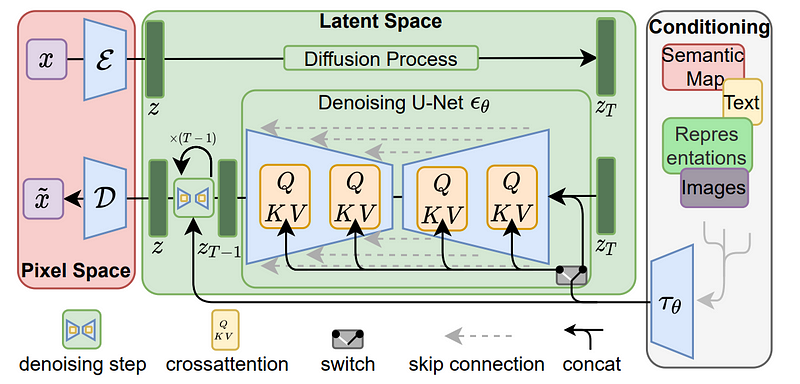
\includegraphics[width=0.8\textwidth]
{static/LDM.png}
\caption{The LDM \cite[Fig.~3]{Rombach_2022_CVPR}.}
\label{fig:ldm}
\end{figure}



\subsubsection{The Autoencoder}
A Variational Autoencoder (VAE) consists of two parts: the encoder and the decoder. "During latent diffusion training, the encoder is used to get the latent representations (latents) of the images for the forward diffusion process, which applies more and more noise at each step" \cite{patil2022stable}. The decoder conversely transforms the denoised latents, created by the U-Net, back into the pixel space at the end of the diffusion process. Only the decoder is used for the image generation process.



\subsubsection{The U-Net}
The U-Net \cite{ronneberger2015u} is a type of Convolutional Neural Network (CNN) that is responsible for predicting the noise in the current sample image. The image generation process starts with a random sample image of gaussian noise. The U-Net then takes this sample \((latents)\) and predicts the noise residual \((noise\_pred)\) of the image. 
A reduced amount (determined by \(sigma\)) of this noise residual is removed in every step, until we end up with the final fully denoised image (see Fig.~\ref{fig:ldm}).
\begin{lstlisting}[language=Python]
latens = latents - sigma * noise_pred
\end{lstlisting}
The U-Net consists of an encoder and a decoder with transformer-based blocks. "Thus, it first encodes the current noised image as a set of tokens, then passes it through a series of transformer blocks" \cite{bolya2023tomesd}. The inclusion of transformer-based blocks allows the model to not only preserve the spacial hierarchies but also the semantic structure of the image.\\
A further aspect that distinguishes the U-Net from an autoencoder are the skip connections that directly pass information from the encoder to the decoder, aiding in the preservation of details during upsampling (see Fig.~\ref{fig:ldm}).



\subsubsection{The Text-Encoder}
The text-encoder is a transformer-based encoder that converts the input prompt from a string to an embedding vector that captures the semantic meaning of text and can be interpreted by the U-Net. Stable Diffusion uses CLIP's \cite{radford2021learning} pre-trained text-encoder \href{https://huggingface.co/docs/transformers/model_doc/clip#transformers.CLIPTextModel}{CLIPTextModel} and thus avoids additional training of the text-encoder.



\subsubsection{The Transformer Block}
Every transformer block has a self-attention (self-attn), cross-attention (cross-attn) and multi-layer perceptron (mlp) module.



\subsubsection*{Self-Attention}
Self-attention \cite{vaswani2017attention} takes a series of (token) vectors and computes outputs while attending to every other token in the sequence. The outputs are generated by first calculating the attention weights between every vector and then taking a weighted sum of the attention weights and the input vectors.
\begin{figure}[!htb]
\centering
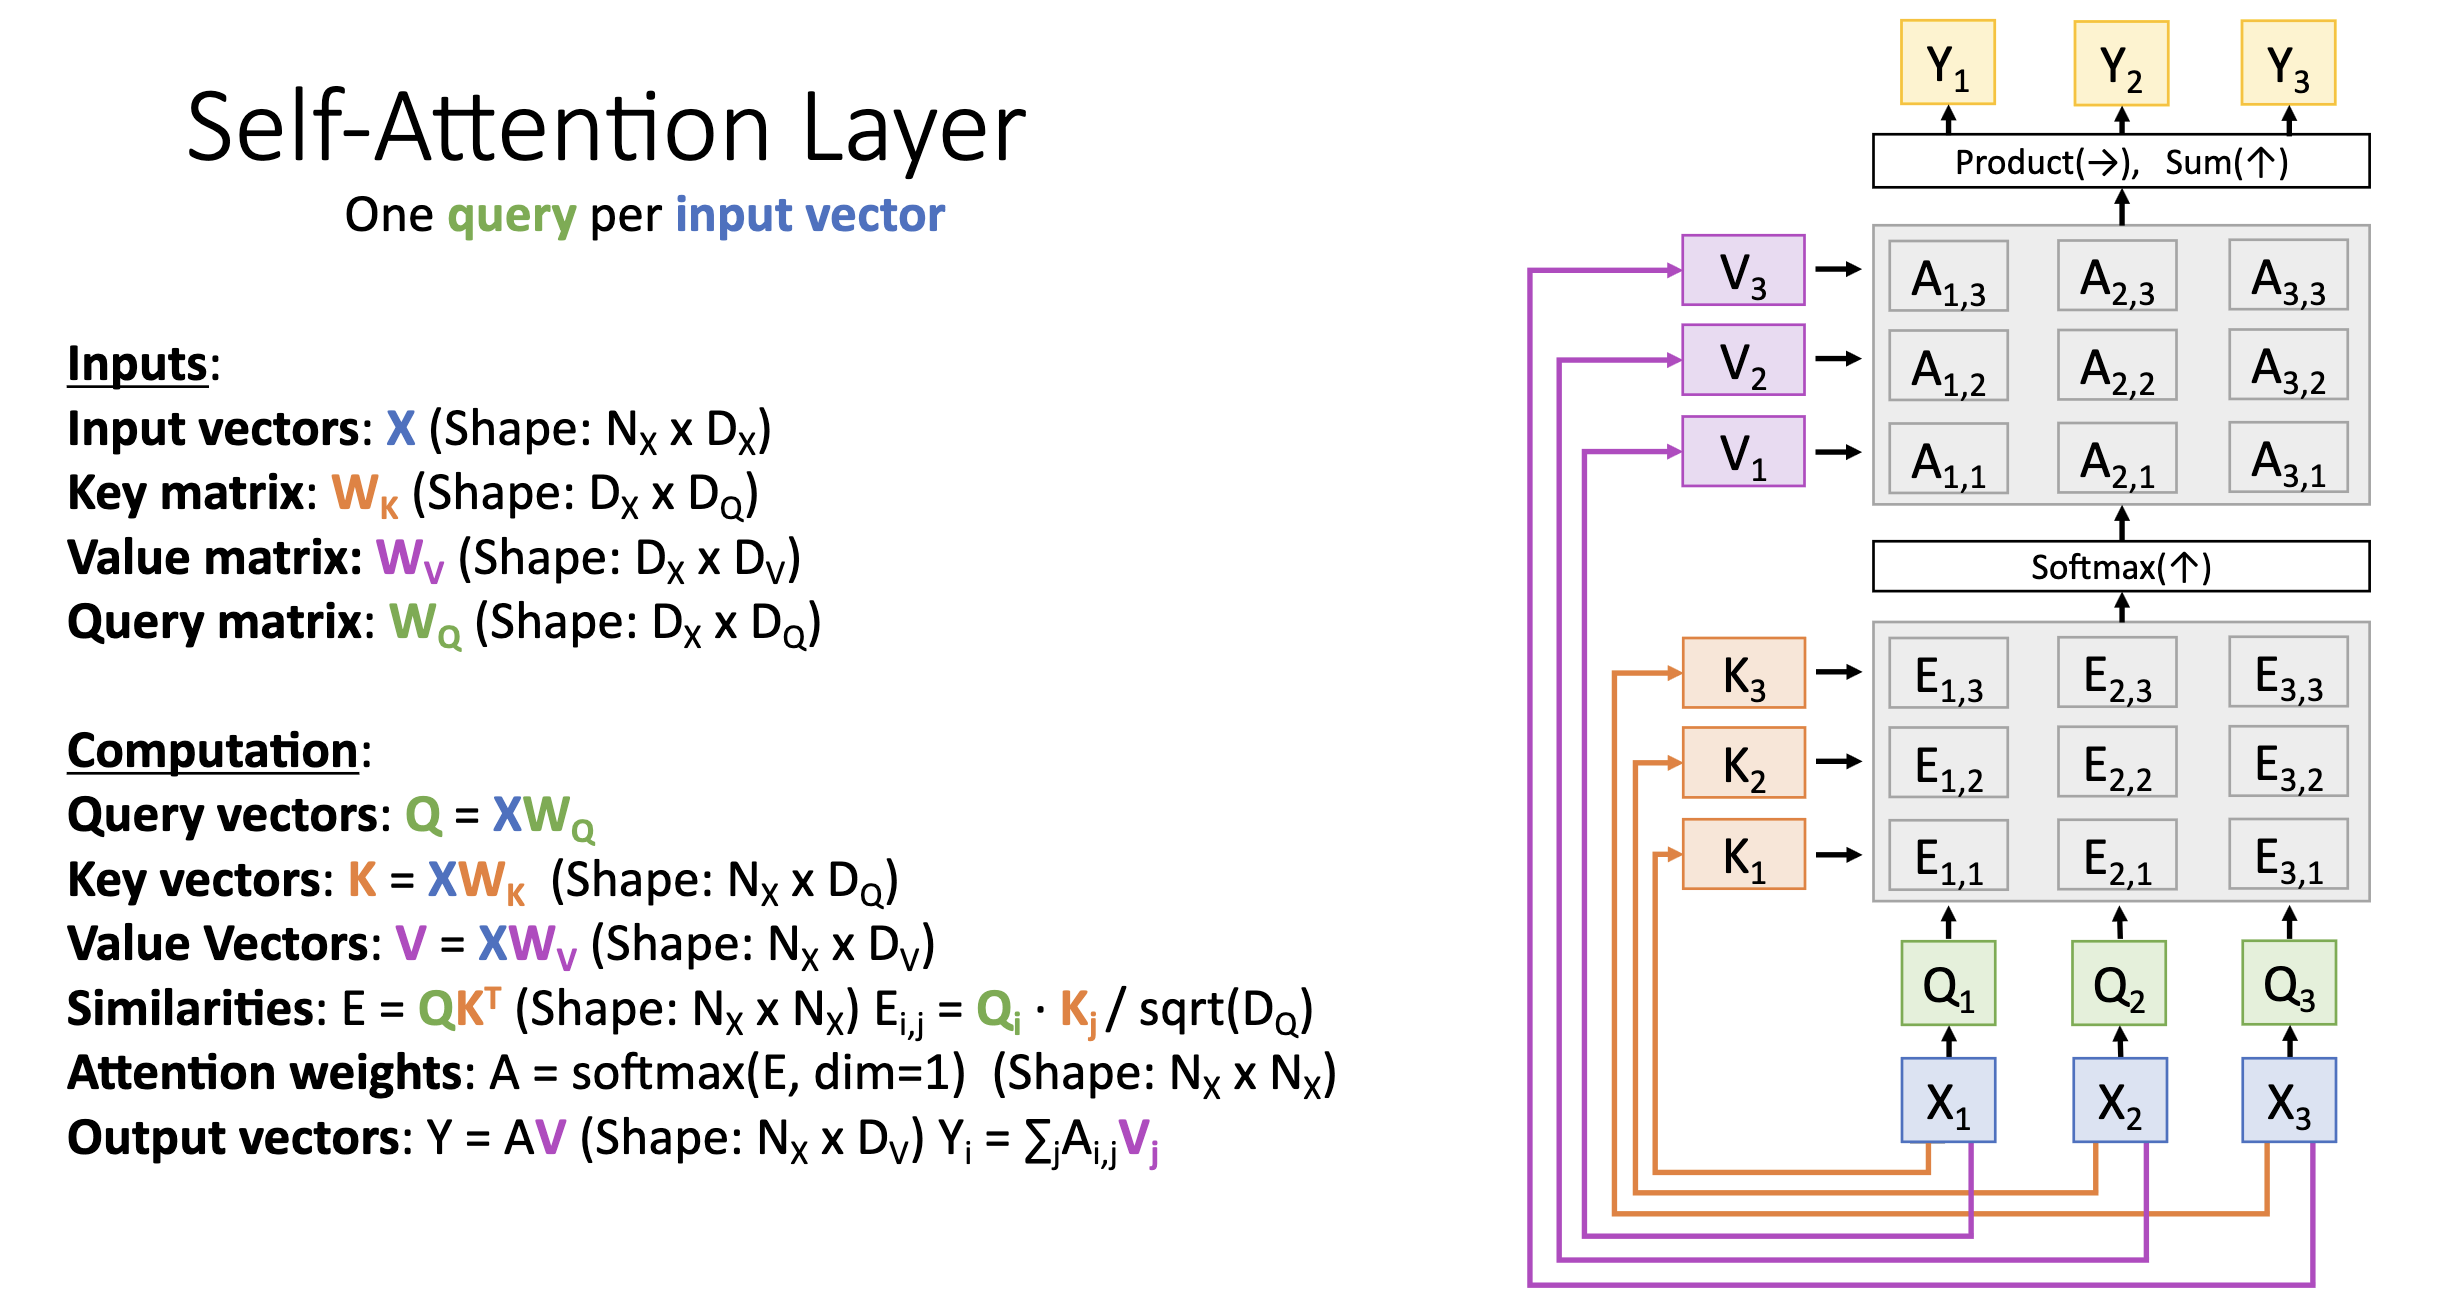
\includegraphics[width=0.95\textwidth]
{static/self_attn.png}
\caption{Self-attention \cite{johnson2019attn}}
\label{fig:self-attn}
\end{figure}

\subsubsection*{Cross Attention}
Text.

\subsubsection*{Multi-Layer Perceptron}
Text.



\subsubsection{Training?}
Forward diffusion. Noise is added to an image. NN trained on it.



\subsection{Frechet-Inception-Distance (FID)}
PyTorch implementation \cite{Seitzer2020FID}



\subsubsection{Inception Model}
Text.




\subsubsection{Caveats}
Inception model is biased. Inception model compresses images to 299x299 pixels. FID inconsistent with ToMe applied (not exactly reproducable)



\subsection{What are Tokens?}
In image synthesis, a token is a block of pixels that are processed collectively by the transformer. Stable Diffusion uses the CLIP tokenizer \cite{radford2021learning} which defines a token as an $14 \times 14$ block of pixels. ---CLIP is trained with the ViT-L/14 model---